\documentclass[final]{beamer}
\mode<presentation>
  {
  \usetheme{Rutgers}
  }
  \usepackage{amsmath,amsthm, amssymb, latexsym}
  \boldmath
  \usepackage[english]{babel}
  \usepackage[latin1]{inputenc}
  \usepackage{lmodern}
  \usepackage[orientation=portrait,size=a0,scale=1.4,debug]{beamerposter}
  
\usepackage{myalgorithm}
\usepackage{wrapfig}
\usepackage[noend]{myalgorithmic}
\usepackage{multirow}
\usepackage{multicol}
\usepackage{graphicx,wrapfig,lipsum}
\usepackage[font=footnotesize]{caption}


  %%%%%%%%%%%%%%%%%%%%%%%%%%%%%%%%%%%%%%%%%%%%%%%%%%%%%%%%%%%%%%%%%%%%%%%%%%%%%%%%%
  \title[Dataset]{Object Detection and Pose Estimation for Robotic Manipulation \\ using Physics Simulation and Monte-Carlo Tree Search}
  \author[Mitash]{Chaitanya Mitash, Abdeslam Boularias and Kostas E. Bekris}
  \institute[RutgersFUES]{Department of Computer Science, Rutgers, the State University of New Jersey}
  %%%%%%%%%%%%%%%%%%%%%%%%%%%%%%%%%%%%%%%%%%%%%%%%%%%%%%%%%%%%%%%%%%%%%%%%%%%%%%%%%
  \newlength{\blocklen}
  \begin{document}
  \setlength{\blocklen}{0.49\textwidth}
  \begin{frame}{} 
    \vspace {-0.5in}
    \begin{columns}[t]
	\begin{column}{0.50\textwidth}
		\begin{block}{\large Motivation for autonomous data generation}
		    	\begin{columns}[T]
		    		\centering
		    		\begin{column}{0.60\textwidth}
					    {\bf \quad Motivation:}
					    \begin{itemize}
						    \item State-of-the-art methods use Convolutional Neural Network (CNN) to perform object segmentation.
						    \item CNNs need access to a large set of labeled data, which requires intensive human labor.
						    \item Current techniques for generating synthetic dataset suffers from dataset bias as they lack realism.
					    \end{itemize}
					    \vspace{0.8in}
					    {\bf\quad Objective:}
					    \begin{itemize}
					    \item Generate a physically-realistic labeled dataset in an autonomous manner to train a CNN for object detection.
					    \end{itemize}
					\end{column}
					\begin{column}{0.40\textwidth}
						\centering
						\vspace{-0.2in}
						\begin{figure}[h]
							\includegraphics[width=0.75\textwidth]{manual_rutgers}
							\vspace{0.1in}
							\caption{Rutgers RGBD dataset with manual annotation}
						\end{figure}
						\vspace{0.3in}
						\begin{figure}[h]
							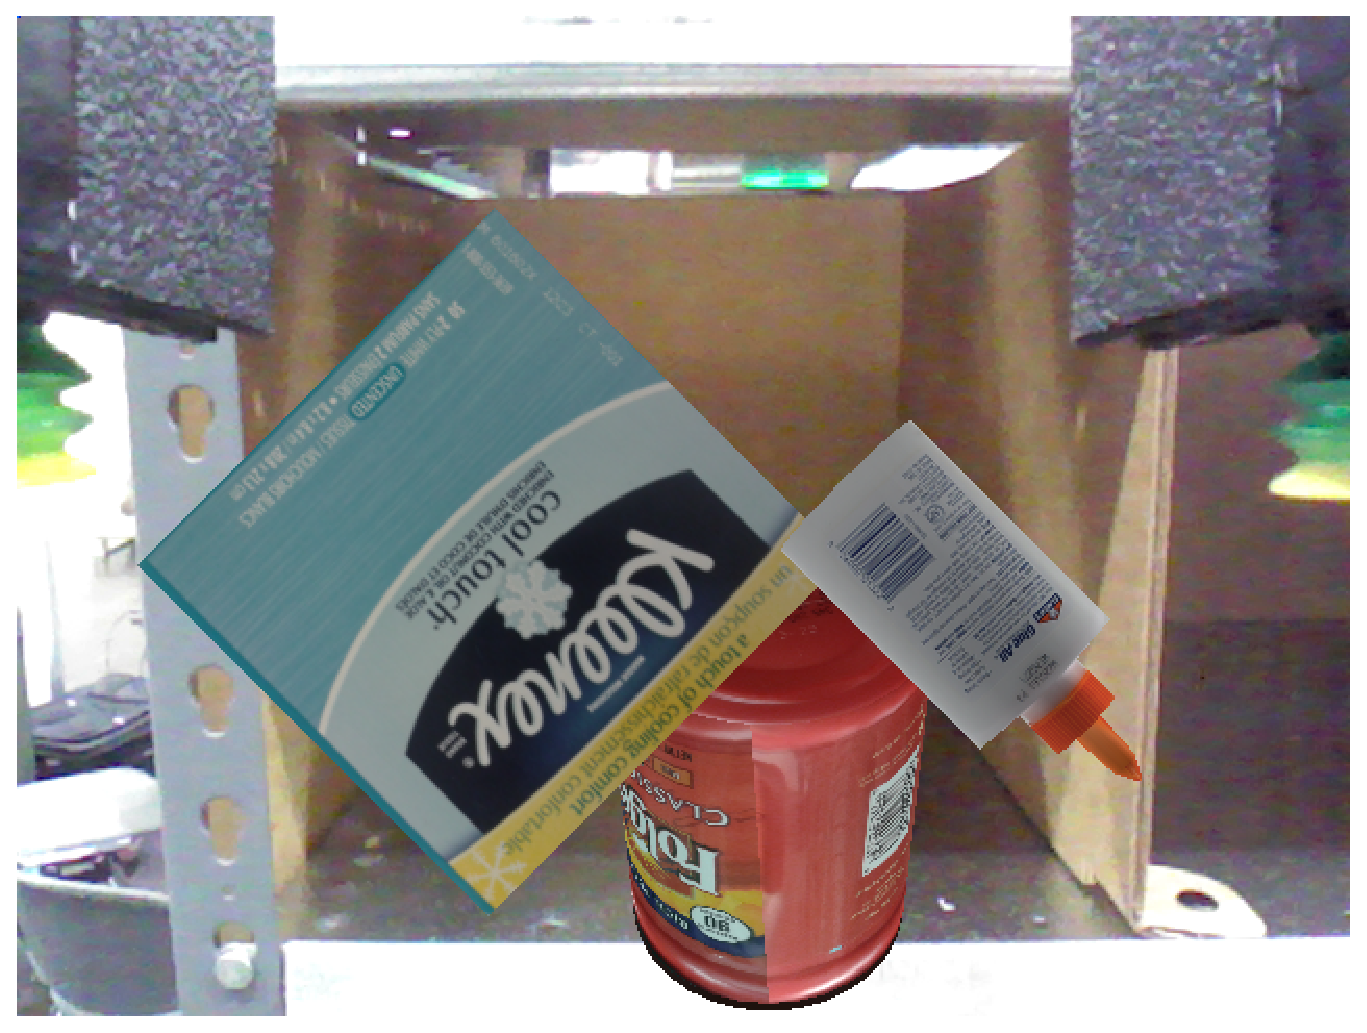
\includegraphics[width=0.75\textwidth]{unreal_syn}
							\vspace{0.1in}
							\caption{Physically unrealistic synthetic dataset generation}
						\end{figure}
					\end{column}
				\end{columns}
		\end{block}
	\end{column}
	\begin{column}{0.50\textwidth}
		\begin{block}{\large Using Physics Simulation to generate training dataset}
		\centering
		    \begin{itemize}
			    \item Environmental and geometric constraints are used to generate datasets for \\setups such as shelf bin and table-top.
			    \item Each scene is generated by randomly sampling object poses from a domain specified for the setup.
			    \item Physics simulation is performed for generating physically realistic scenes so that the training dataset captures appropriate object scales and occlusions.
		    \end{itemize}
		    \vspace{0.2in}
		    \begin{figure}[h]
				\includegraphics[width=0.80\textwidth]{physim}
				\caption{Pipeline for data generation using physics simulation}
			\end{figure}
		\end{block}
	\end{column}
\end{columns}	
		    

    \vfill
    
\begin{columns}[t]
	\begin{column} {0.32\textwidth}
		\begin{block}{\large Data Collection}
			\centering
				\vspace{0.2in}
				\begin{figure}[h]
					\includegraphics[width=0.8\textwidth]{datacollectionsetup_2}
					\caption{Our data collection hardware and environment}
				\end{figure}
				% \vspace{0.1in}
					\begin{columns}[t]
						\begin{column}{0.94\textwidth}
							\begin{itemize}
								\item Collection performed on Motoman Dual-arm SDA10F humanoid robot using Kinect v1 RGBD camera
								\item Camera located on wrist of robot, position calibrated prior to data collection
								\item 10,368 RGBD images collected involving 24 target objects, each shown in:
									\begin{itemize}
										\item 12 different bin locations
										\item 3 clutter states per bin (1, 2, 3 items)
										\item 3 viewpoints per clutter state
										\item 4 frames per viewpoint
									\end{itemize}
								\item 6D Ground truth annotated by hand, including all transformations between object, camera, and robot base
							\end{itemize}
						\end{column}
					\end{columns}
				\vspace{0.1in}
		\end{block}
		% \begin{block}{\large Monotone Method by Stilman et al. '07}
		% 	\begin{itemize}
		% 		\item Adaptation of previous work for solving rearrangement tasks.
		% 		\item Backtracking search for monotone problems.
		% 		\item Computationally fast even upon failure.
		% 		\item Requirement: no overlapping initial and target poses. 			 
		% 	\end{itemize}
		% 	\centering
		% 	% \includegraphics [width=0.43\blocklen] {monotone1} \hspace {0.5in}
		% 	% \includegraphics [width=0.43\blocklen] {monotone2}
		% \end{block}
	\end{column}
	%Second general Column
	\begin{column}{0.68\textwidth}
		\begin{block} {\large Dataset Features}
			\begin{columns}[T]
				\centering
				\begin{column}{0.59\textwidth}
					\begin{itemize}
						\item Large dataset covering wide variety of objects with 6D ground truth object pose annotatations
						\item Good sample coverage of probable object poses within the shelves
						\item Provides researchers the ability to determine the effects of immediate clutter on pose estimation
							\begin{itemize}
								\item Same ground truth target object pose is given with varying degrees of clutter within the bin
							\end{itemize}
						\item Allows opportunity to analyze accuracy based on the camera's viewpoint
							\begin{itemize}
								\item For each shelf configuration, samples are generated from 3 different viewing positions
							\end{itemize}
						\item Provides the ability to determine the effects of slight sensor noise on deterministic algorithms
							\begin{itemize}
								\item For each shelf configuration at each viewpoint 4 samples are generated
							\end{itemize}
					\end{itemize}
					
				\end{column}
				\begin{column}{0.40\textwidth}
					\centering
					\begin{figure}[h]
						\includegraphics[width=0.8\textwidth]{shelf_positions}
						\caption{Variety of coverage in our dataset of ground truth poses for a single object}
					\end{figure}
				\end{column}
			\end{columns}
			\hspace{0.02\textwidth}
			\begin{figure}[h]
				\includegraphics[width=0.3\textwidth]{munchkin_1} \hspace{0.02\textwidth}
				\includegraphics[width=0.3\textwidth]{munchkin_2} \hspace{0.02\textwidth}
				\includegraphics[width=0.3\textwidth]{munchkin_3} 
				\caption{Examples from our dataset showing the same target object pose (the ``duck'') in varying degrees of clutter within the bin}
			\end{figure}
		\end{block}
		% \begin{block}{\large Non-monotone Extension}
		% 	\begin{itemize}
		% 		\item Evacuate the blocking objects to intermediate poses. 
		% 		\item Solve Minimum Constraint Removal Problem to detect intermediate poses.
		% 		\item Requirement: Enough space to move blocking objects.
		% 	\end{itemize}
		% 	\begin{columns}[T]
		% 		\begin{column}{0.48\blocklen}
		% 			\centering
		% 			% \includegraphics [width=0.45\blocklen] {nonmonotone1}
		% 			{\small
		% 			\begin{itemize}
		% 				\item The method works regardless the order with which objects are evacuated.
		% 			\end{itemize}
		% 			}
		% 		\end{column}
		% 		\begin{column}{0.48\blocklen}
		% 			\centering
		% 			% \includegraphics [width=0.45\blocklen] {nonmonotone2}
		% 			{\small
		% 			\begin{itemize}
		% 				\item Backward search for detecting a valid sequence of objects evacuations.  
		% 			\end{itemize}
		% 			}
		% 		\end{column}
		% 	\end{columns}
		% \end{block}
	\end{column}
\end{columns}




    \vfill
    \begin{columns}[t]
	\begin{column}{0.70\textwidth}
		\begin{block}{\large Pose Estimation using Monte Carlo Tree Search}
			\centering
			\begin{figure}[h]
				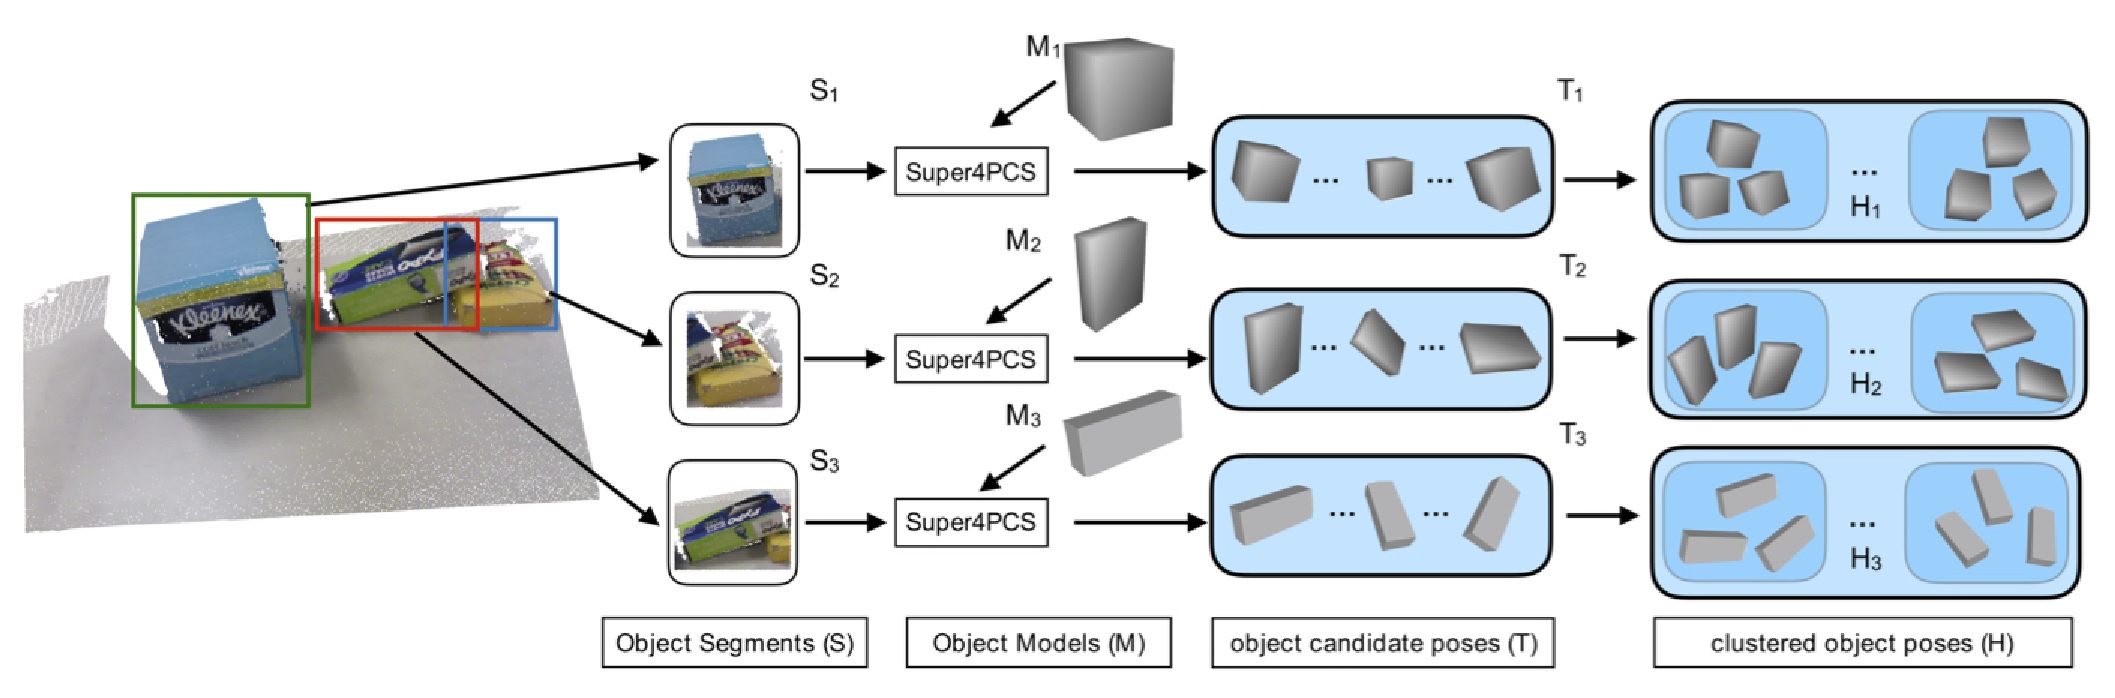
\includegraphics[width=0.9\textwidth]{clustering}
				\caption{object candidate pose generation and clustering to reduce set cardiniality}
			\end{figure}
			\vspace{-0.3in}
			\begin{itemize}
				\item Pose candidate set is constructed for each object using the extracted object segment and the 3D CAD model.
				\item For computational efficiency, the set of object hypotheses is clustered to obtain smaller candidate sets while still containing poses close to the true solutions. 
			\end{itemize}
			\vspace{-0.3in}
			\begin{columns}[t]
			\begin{column} {0.40\textwidth}
			\begin{figure}[h]
				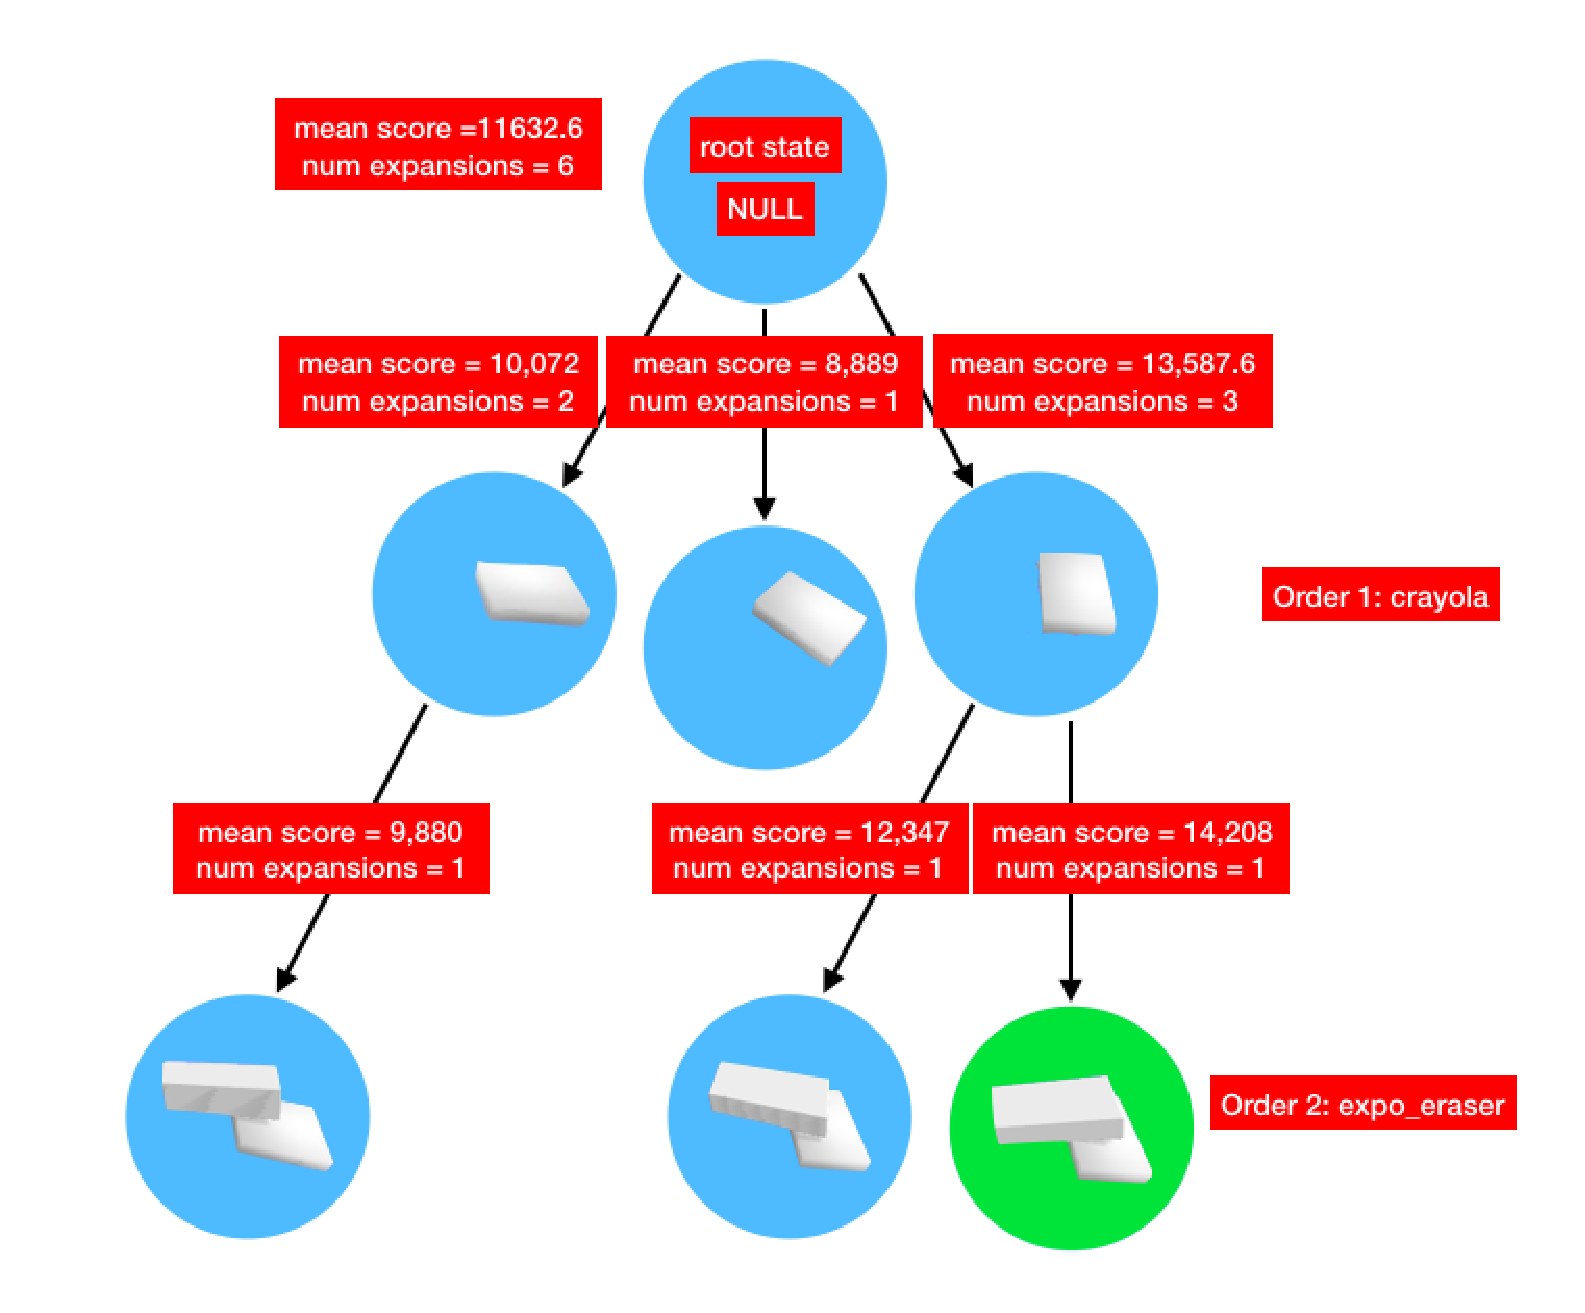
\includegraphics[width=0.8\textwidth]{mcts}
				\caption{Monte Carlo Tree Search for pose estimation}
			\end{figure}
			\end{column}
			\begin{column} {0.60\textwidth}
			\begin{itemize}
				\item An order of object placement is computed based on a set of rules defined over the object segments.
				\item Node expansion in the tree corresponds to an object placement, which is constrained (imposed by using physics simulator and point cloud trimming) by the previously placed objects.
				\item The leaf nodes (complete assignment) are rendered and a score is computed by comparing rendered scene to the observed depth image.
				\item The search uses Upper Confidence Bound to trade-off exploration and exploitation within the search.
			\end{itemize}
			\end{column}
			\end{columns}
		\end{block}
	\end{column}
	\begin{column}{0.30\textwidth}
		\begin{block}{\large Pose Estimation Evaluation}
			\centering
			\begin{itemize}
				\item Results demonstrate that search is useful in case of a clutter.
				\item MCTS converges much faster compared to using a heuristic based on registration score.
			\end{itemize}
			\vspace{-0.2in}
			\begin{figure}[h]
				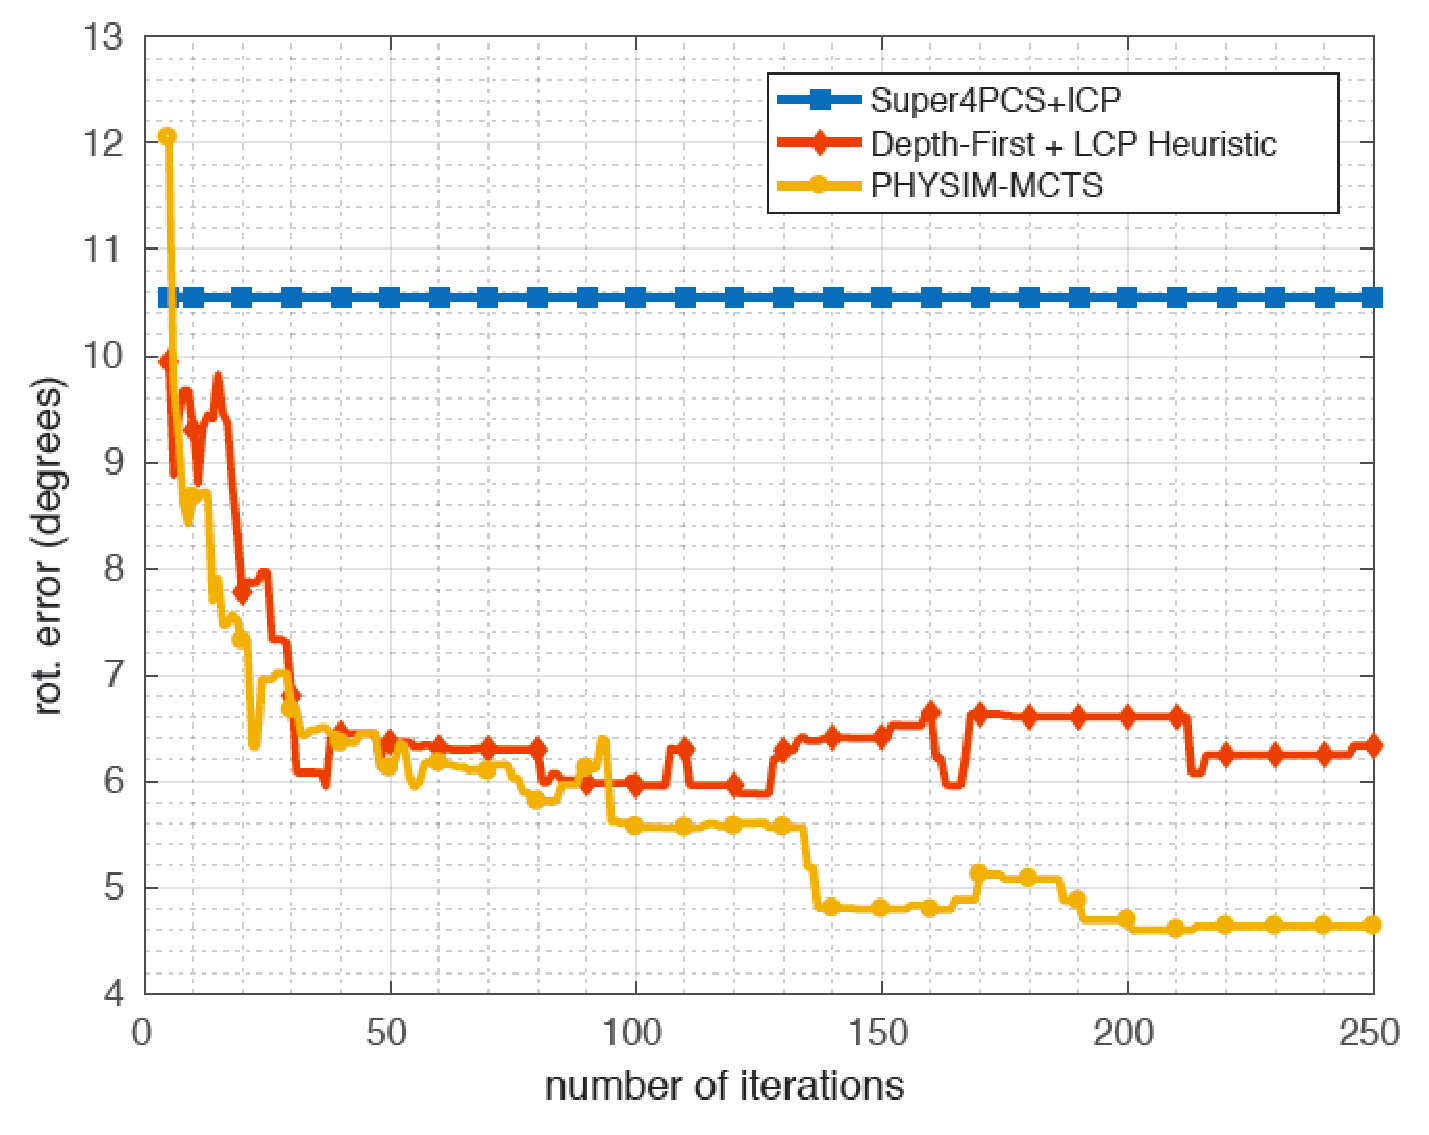
\includegraphics[width=0.75\textwidth]{graph1}
				\caption{Rotation error (degrees) vs the number of search expansions}
			\end{figure}
			\begin{figure}[h]
				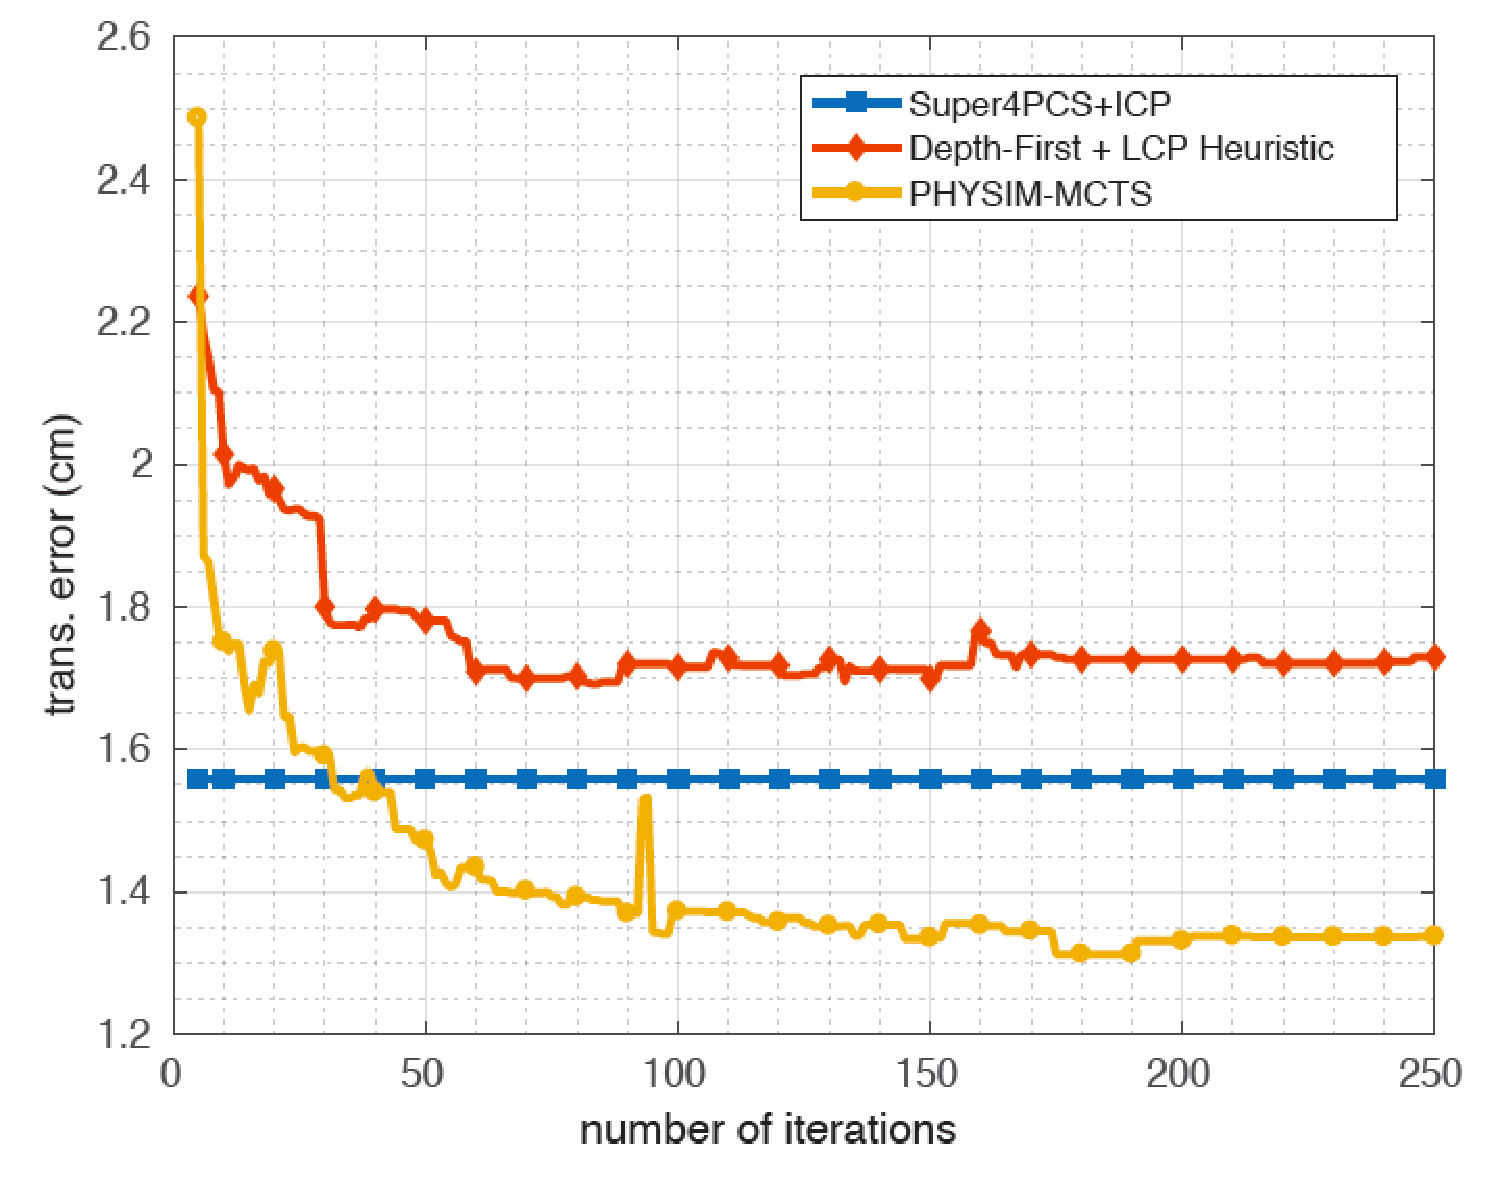
\includegraphics[width=0.75\textwidth]{graph2}
				\caption{Translational error (cms) vs the number of search expansions}
			\end{figure}
		\end{block}
	\end{column}
\end{columns}
    \vfill
  \end{frame}
\end{document}


%%%%%%%%%%%%%%%%%%%%%%%%%%%%%%%%%%%%%%%%%%%%%%%%%%%%%%%%%%%%%%%%%%%%%%%%%%%%%%%%%%%%%%%%%%%%%%%%%%%%
%%% Local Variables: 
%%% mode: latex
%%% TeX-PDF-mode: t
%%% End:
